\chapter{Technische Grundlagen}
\label{cha:technische-grundlagen}

Dieses Kapitel bietet einen Überblick über die wichtigsten technischen Konzepte und Methoden, die für das Verständnis moderner Dokumentenverarbeitungssysteme grundlegend sind. Dabei werden sowohl grundlegende Konzepte als auch Metriken zur Messung des Erfolgs bearbeitet. 

\section{Optical Character Recognition (OCR)}
\label{sec:optical-character-recognition-ocr}

\gls{OCR} spielt eine Schlüsselrolle bei der Verarbeitung visueller Dokumente. 
Sie wandelt Bilder von gedrucktem oder handgeschriebenem Text in maschinenlesbaren Text um \cite{MoriS.1992HroO}.
Entgegen der wörtlichen Bedeutung von \gls{OCR} arbeiten viele gängige Systeme tatsächlich auf Zeichenblöcke oder ganze Wörter anstatt einzelner Zeichen \cite{BorovikovEugene2014Asom}.
Es existiert eine Vielzahl von \gls{OCR}-Methoden, von denen einige Segmentierung nutzen, also die Zuteilung jedes Pixels zu einer Kategorie, während andere darauf verzichten \cite{BorovikovEugene2014Asom}. 
Die meisten modernen \gls{OCR}-Systeme bestehen typischerweise aus zwei essenziellen Komponenten \cite{BorovikovEugene2014Asom}:

\begin{enumerate}
	\item Feature Extractor: Dieser extrahiert die charakteristischen Merkmale (Deskriptoren) eines Elements aus einem Bild. Diese abgeleiteten Merkmale dienen als Eingabe für den Classifier.
	\item Classifier: Anhand der extrahierten Merkmale bestimmt dieser das (wahrscheinlichste) bekannte Element. Zusätzlich liefert der Klassifikator einen Konfidenzwert, der die Sicherheit der Elementerkennung angibt.
\end{enumerate}

Diese grundlegende Struktur bildet die Basis für verschiedene klassische und moderne Methoden der optischen Zeichenerkennung \cite{BorovikovEugene2014Asom}:

\begin{itemize}
	\item Template Matching: Vergleicht Eingabezeichen pixelweise mit bekannten Vorlagen und wählt die ähnlichste aus.
	\item Strukturelle Klassifikation: Nutzt strukturelle Merkmale wie Striche, Löcher oder Ecken und wendet regelbasierte Systeme an.
\end{itemize}

Dabei ist zu beachten, dass es auch leichte Abweichungen und hybride Varianten dieser Techniken gibt \cite{BorovikovEugene2014Asom}. Viele moderne \gls{OCR}-Systeme verwenden mathematische Funktionen, die darauf abzielen, eine Metrik der Abweichung von einer Vorlage zu minimieren. Beispiele dafür sind \cite{BorovikovEugene2014Asom}:

\begin{itemize}
	\item Diskriminanzfunktionen: Diese verwenden Hyperebenen im mehrdimensionalen Merkmalsraum zur Trennung von Zeichenklassen.
	\item Bayes-Klassifikatoren: Sie minimieren Fehlklassifikationen mittels Wahrscheinlichkeitstheorie.
	\item Künstliche Neuronale Netze (KNN): Diese lernen komplexe Klassifikationsabbildungen durch Fehlerrückführung und Optimierungstechniken.
\end{itemize}

\subsection{Tesseract OCR}
\label{subsec:tesseract-ocr}

Das für die im Rahmen dieser Bachelorarbeit implementierten Prototypen verwendete \gls{OCR}-System heißt Tesseract \gls{OCR}. Hewlett Packard entwickelte dieses \gls{OCR}-System ursprünglich, und seit 2005 ist es als Open-Source-Software verfügbar \cite{SmithR_2007_AOot}. Tesseract basiert auf \gls{LSTM} neuronalen Netzen und unterstützt über 100 Sprachen sowie mehr als 35 Schriftsysteme \cite{tesseract_ocr_user_manual}. 

\subsubsection{Architektur und Funktionsweise}
\label{subsubsec:architektur-und-funktionsweise}

Tesseract folgt einem traditionellen Pipeline-Ansatz für die Texterkennung, wobei einige Schritte zur Zeit ihrer Entwicklung innovativ waren \cite{SmithR_2007_AOot}. Der Prozess beginnt mit einer Analyse verbundener Komponenten, bei der das System die Umrisse der Komponenten speichert. Diese Methode ermöglicht es Tesseract, sowohl schwarzen Text auf weißem Hintergrund als auch umgekehrt zu erkennen \cite{SmithR_2007_AOot}.

\subsubsection{Zeilenfindung und Basislinienanpassung}
\label{subsubsec:zeilenfindung-und-basislinienanpassung}

Ein wichtiger Aspekt von Tesseract ist der Algorithmus zur Zeilenfindung. Dieser ermöglicht es, schiefe Seiten ohne vorherige Entzerrung zu erkennen, was einen Qualitätsverlust des Bildes verhindert \cite{SmithR_2007_AOot}. Nach der Zeilenerkennung passt das System die Basislinien präzise an. Diese Fähigkeit erlaubt es Tesseract, auch mit gekrümmten Basislinien umzugehen – ein häufiges Problem beim Scannen von Büchern \cite{SmithR_2007_AOot}.

\subsubsection{Zeichenerkennung und Klassifizierung}
\label{subsubsec:zeichenerkennung-und-klassifizierung}

Tesseract verwendet einen zweistufigen Klassifizierungsprozess, um sich auf die jeweilige Schriftart sowie mögliche Artefakte anzupassen \cite{SmithR_2007_AOot}:

\begin{enumerate}
	\item Ein schneller Vorfilter erstellt zunächst eine Liste möglicher Zeichenklassen.
	\item Für diese Auswahl führt das System anschließend eine genauere Ähnlichkeitsberechnung durch.
\end{enumerate}

Diese Methode kombiniert Effizienz und Genauigkeit. 

Zusätzlich nutzt Tesseract einen adaptiven Klassifizierer. Dieser lernt während des Erkennungsvorgangs kontinuierlich dazu und passt sich so an die spezifischen Eigenschaften des aktuellen Dokuments an. Er verwendet die gleichen Grundlagen wie der Hauptklassifizierer, normalisiert die Eingabedaten jedoch anders. Diese Anpassung verbessert die Erkennung von Groß- und Kleinbuchstaben und verringert die Störungsanfälligkeit \cite{SmithR_2007_AOot}.

Die Kombination aus effizientem zweistufigem Prozess und anpassungsfähigem Lernen ermöglicht Tesseract eine genaue Texterkennung in verschiedenen Dokumenttypen und Schriftstilen.

\section{Grundlagen des maschinellen Lernens}
\label{sec:grundlagen-des-maschinellen-lernens}

\gls{ML} ist ein Teilbereich der Informatik, der sich mit der Entwicklung von Algorithmen und Techniken zur Automatisierung komplexer Problemlösungen befasst \cite{RebalaGopinath2019AItM}. \gls{ML}-Algorithmen lernen aus Daten, ohne explizit programmiert zu werden. Der Hauptunterschied zur konventionellen Programmierung besteht darin, dass \gls{ML} selbstständig Regeln aus Beispieldaten ableitet, anstatt einem vordefinierten Regelwerk zu folgen.

Forscher*innen unterscheiden verschiedene Arten von Lernvorgängen \cite{RebalaGopinath2019AItM, jordan2015machine}:

\begin{itemize}
	\item Überwachtes Lernen (Supervised Learning):Der Algorithmus lernt anhand von gelabelten Trainingsdaten. Klassifikations- und Regressionsaufgaben sind typische Anwendungsbeispiele.
	\item Unüberwachtes Lernen (Unsupervised Learning): Der Algorithmus entdeckt Muster in ungelabelten Daten; wie beispielsweise beim Clustering.
	\item Semi-überwachtes Lernen (Semi-supervised Learning): EDieses Verfahren kombiniert gelabelte und ungelabelte Daten. Es findet häufig Anwendung bei einem Mangel an gelabelten Daten.
	\item Verstärkendes Lernen (Reinforcement Learning): Der Algorithmus lernt durch Interaktion mit einer Umgebung und erhält Belohnungen für bestimmte Aktionen.
\end{itemize}

Die beeindruckenden Fortschritte im Bereich des \gls{ML} in den letzten Jahren sind auf verschiedene Faktoren zurückzuführen, darunter die Verfügbarkeit großer Datenmengen, die Zunahme der Rechenleistung und verbesserte Algorithmen für große Datensätze \cite{jordan2015machine}.

Im Rahmen von \gls{ML} gibt es verschiedene Unterarten, welche in den folgenden Absätzen besprochen werden, einen Überblick darüber bietet die Abbildung \ref{fig:ml-hierarchy}.

\begin{figure}[h]
	\centering
	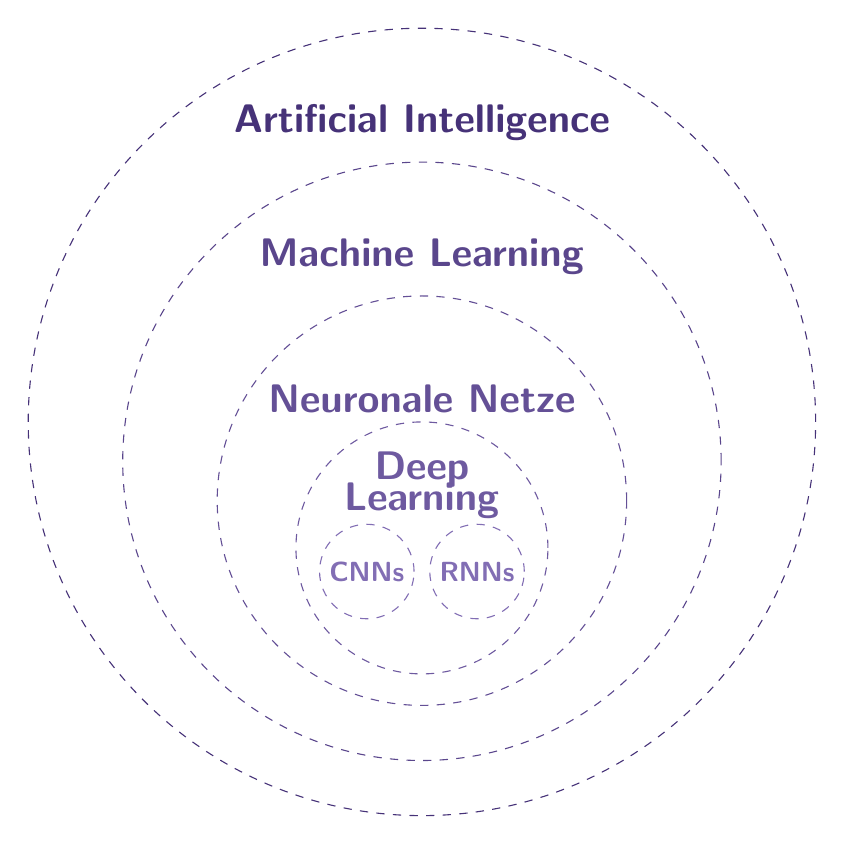
\begin{tikzpicture}[font=\sffamily]
		% Define colors
		\definecolor{outercolor}{RGB}{70,50,120}
		\definecolor{middlecolor}{RGB}{90,70,140}
		\definecolor{innermiddlecolor}{RGB}{100,80,150}
		\definecolor{innercolor}{RGB}{110,90,160}
		\definecolor{innermostcolor}{RGB}{130,110,180}
		% Outer circle (Artificial Intelligence)
		\draw[dashed, outercolor] (0,0) circle (5cm);
		\node[outercolor] at (0,3.8) {\Large\textbf{Artificial Intelligence}};
		% Middle circle (Machine Learning)
		\draw[dashed, middlecolor] (0,-0.5) circle (3.8cm);
		\node[middlecolor] at (0, 2.1) {\Large\textbf{Machine Learning}};
		% Inner-middle circle (Neuronale Netze)
		\draw[dashed, innermiddlecolor] (0,-1) circle (2.6cm);
		\node[innermiddlecolor] at (0,0.3) {\Large\textbf{Neuronale Netze}};
		% Inner circle (Deep Learning)
		\draw[dashed, innercolor] (0,-1.6) circle (1.6cm);
		\node[innercolor] at (0,-0.6) {\Large\textbf{Deep}};
		\node[innercolor] at (0,-1) {\Large\textbf{Learning}};
		% Innermost circles (CNNs and RNNs)
		\draw[dashed, innermostcolor] (-0.7,-1.9) circle (0.6cm);
		\node[innermostcolor] at (-0.7,-1.9) {\textbf{CNNs}};
		\draw[dashed, innermostcolor] (0.7,-1.9) circle (0.6cm);
		\node[innermostcolor] at (0.7,-1.9) {\textbf{RNNs}};
	\end{tikzpicture}
	\caption{Zusammenhang von \glspl{ML}, neuronalen Netzen, Deep Learning, \glspl{CNN} und \glspl{RNN}}
	\label{fig:ml-hierarchy}
\end{figure}

\subsection{Neuronale Netze}
\label{subsec:neuronale-netze}

Neuronale Netze bilden eine Klasse von \gls{ML}-Modellen, die sich von der Funktionsweise des menschlichen Gehirns inspirieren lassen \cite{RebalaGopinath2019AItM}. Sie bestehen aus miteinander verbundenen Neuronen, die in Schichten angeordnet sind:

\begin{itemize}
	\item Eingabeschicht (Input Layer): Nimmt die Eingabedaten auf
	\item Versteckte Schichten (Hidden Layer): Verarbeiten die Informationen
	\item Ausgabeschicht (Output Layer): Liefert das Ergebnis
\end{itemize}

Die Verbindungen zwischen den Neuronen besitzen Gewichte, die sich während des Trainings anpassen. Durch nichtlineare Aktivierungsfunktionen können neuronale Netze komplexe Zusammenhänge modellieren.

\subsubsection{Deep Learning}
\label{subsec:deep-learning}

Deep learning bezeichnet neuronale Netze mit vielen versteckten Schichten \cite{RebalaGopinath2019AItM}. Diese Architektur ermöglicht die Extraktion hierarchischer Merkmale aus den Daten. Die Entwicklung von Algorithmen für tiefes Lernen führte in den letzten Jahren zu großen Fortschritten in Bereichen wie Bilderkennung, Sprachverarbeitung, Robotik und \gls{OCR} \cite{jordan2015machine}.

Wichtige Konzepte im Deep Learning sind:

\begin{itemize}
	\item Backpropagation: Ein Algorithmus zum effizienten Training durch Berechnung der Gradienten \cite{RebalaGopinath2019AItM}
	\item Regularisierung: Techniken zur Vermeidung von Overfitting \cite{jordan2015machine}
	\item Transfer Learning: Übertragung gelernter Merkmale auf neue Aufgaben \cite{jordan2015machine}
\end{itemize}

\subsubsection{Convolutional Neural Networks (CNNs)}
\label{subsubsec:cnn}

\glspl{CNN} stellen eine spezielle Art von neuronalen Netzen dar, die sich besonders für die Verarbeitung von Bilddaten eignen \cite{RebalaGopinath2019AItM}. Sie nutzen Faltungsoperationen (Convolutions), um lokale Muster in den Eingabedaten zu erkennen. Im Kontext von \glspl{CNN} unterscheiden wir verschiedene gängige Ebenentypen \cite{RebalaGopinath2019AItM}:

\begin{itemize}
	\item Convolutional Layer: Wendet Filter (Kernel) zur Merkmalserkennung an
	\item ReLU (Rectified Linear Unit): Führt nach einer Faltungsschicht nichtlineare Merkmale ein und setzt negative Werte auf Null, um die Komplexität des Modells zu reduzieren
	\item Pooling Layer: Reduziert die räumlichen Dimensionen
	\item Fully Connected Layer: Verbindet jedes Neuron mit allen Neuronen der vorhergehenden Schicht; führt Klassifikation basierend auf extrahierten Merkmalen durch
\end{itemize}

CNNs haben sich als äußerst leistungsfähig für Aufgaben wie Objekterkennung, Gesichtserkennung und autonomes Fahren erwiesen \cite{RebalaGopinath2019AItM}. Ihre Fähigkeit, hierarchische Merkmale aus Bilddaten zu extrahieren, macht sie zu einem zentralen Werkzeug in vielen Bereichen der künstlichen Intelligenz.

\section{Natural Language Processing (NLP)}
\label{sec:nlp}

\gls{NLP} beschäftigt sich mit dem Verstehen und der Interpretation menschlicher Sprache, sowohl gesprochen als auch geschrieben, mithilfe maschineller Verarbeitung \cite{RebalaGopinath2019AItM}. \gls{NLP} findet Anwendung in einer Vielzahl von Bereichen, darunter Spracherkennung, Übersetzungen, Textzusammenfassungen, Fragebeantwortung, Spracherzeugung und Suchmaschinen.

\subsection{Tokenisierung}
\label{subsec:tokenisierung}

Die Tokenisierung bildet einen fundamentalen Schritt in der Verarbeitung natürlicher Sprache. Hierbei wird ein Text in einzelne Einheiten, sogenannte Token, zerlegt \cite{RebalaGopinath2019AItM}. In den meisten Fällen entsprechen diese Token einzelnen Wörtern, sie können aber auch Satzzeichen oder andere bedeutungstragende Elemente umfassen \cite{RebalaGopinath2019AItM}. 
Ein einfacher Ansatz für englische Texte besteht beispielsweise darin, den Text an Leerzeichen zu trennen.

\subsection{Part-of-Speech Tagging}
\label{subsec:pos-tagging}

Im \gls{POS}-Tagging-Schritt wird jedes Wort in einem Text einer grammatikalischen Kategorie zugeordnet, wie zum Beispiel Nomen, Verb oder Adjektiv \cite{RebalaGopinath2019AItM}. Dieser Schritt ist von großer Bedeutung, da die grammatikalische Funktion eines Wortes oft entscheidend für seine Bedeutung im Kontext ist.

\subsection{Named Entity Recognition}
\label{subsec:ner}

\gls{NER} ist eine zentrale Aufgabe im \gls{NLP}, bei der es darum geht, benannte Entitäten in einem Text zu identifizieren und zu klassifizieren \cite{nadeau2007survey}. 
Typische benannte Entitäten umfassen Eigennamen von Personen, Organisationen und Orten, aber auch Zeitangaben, Währungen und andere spezifische Bezeichnungen.

\gls{NER}-Systeme müssen in der Lage sein, mehrdeutige Begriffe korrekt zu interpretieren. So kann "Tesla" je nach Kontext als Personenname, Unternehmensname oder als Einheit für magnetische Flussdichte verstanden werden \cite{RebalaGopinath2019AItM}.

Die Entwicklung von \gls{NER}-Systemen hat verschiedene Ansätze hervorgebracht:

\begin{itemize}
	\item Regelbasierte Systeme: Frühe \gls{NER}-Systeme basierten hauptsächlich auf manuell erstellten Regeln und Wörterbüchern \cite{nadeau2007survey}.
	\item Maschinelles Lernen: Moderne Ansätze nutzen zunehmend maschinelle Lernverfahren, insbesondere überwachtes Lernen. Dabei trainieren Forscher*innen Modelle auf großen, annotierten Texten, um Muster und Kontexte zu erkennen, die auf benannte Entitäten hindeuten \cite{nadeau2007survey}.
	\item Hybride Ansätze: Diese kombinieren die Flexibilität des maschinellen Lernens mit domänenspezifischem Wissen \cite{nadeau2007survey}. Dieser Ansatz hat sich als besonders effektiv erwiesen und verbessert die Genauigkeit der Erkennung.
\end{itemize}

\subsection{Transformer-Architektur}
\label{subsec:transformer-architecture}

Die Transformer-Architektur, erstmals von \textcite{VaswaniAshish2023AIAY} vorgestellt, revolutionierte das Feld des maschinellen Lernens für natürliche Sprache. Im Gegensatz zu früheren rekurrenten oder faltungsbasierten Modellen basiert der Transformer vollständig auf Aufmerksamkeitsmechanismen (Attention), was eine effizientere Verarbeitung langer Sequenzen ermöglicht.

Kernelemente der Transformer-Architektur umfassen \cite{VaswaniAshish2023AIAY}:

\begin{itemize}
	\item Multi-Head Attention: Ermöglicht dem Modell, verschiedene Aspekte der Eingabe parallel zu berücksichtigen.
	\item Positionscodierung: Fügt Informationen über die Reihenfolge der Tokens hinzu, da die Attention-Mechanismen selbst keine Reihenfolge berücksichtigen.
	\item Feed-Forward-Netzwerke: Verarbeiten die Ausgaben der Attention-Layer weiter.
	\item Residuale Verbindungen und Layer-Normalisierung: Verbessern den Informationsfluss und stabilisieren das Training.
\end{itemize}

Die Transformer-Architektur hat sich aufgrund ihrer Skalierbarkeit und Effizienz als Grundlage für viele moderne Sprachmodelle etabliert \cite{VaswaniAshish2023AIAY}.

\subsection{BERT und verwandte Modelle}
\label{subsec:bert-und-verwandte-modelle}

Die von \textcite{DevlinJacob2019BPoD} vorgestellte \gls{BERT}-Technologie markierte einen weiteren bedeutenden Fortschritt in der Anwendung von Transformer-Architekturen. BERT verwendet eine bidirektionale Vortrainingsmethode, die es dem Modell ermöglicht, Kontext aus beiden Richtungen zu berücksichtigen \cite{DevlinJacob2019BPoD}.

Wichtige Aspekte dieses Trainingsprozesses sind \cite{DevlinJacob2019BPoD}:

\begin{itemize}
	\item \gls{MLM}: Trainiert das Modell, maskierte Wörter in einem Satz vorherzusagen.
	\item \gls{NSP}: Trainiert das Modell, die Beziehung zwischen Satzpaaren zu verstehen.
\end{itemize}

\gls{BERT} \cite{DevlinJacob2019BPoD} sowie Varianten wie ALBERT \cite{LanZhenzhong2019AALB} oder RoBERTa \cite{liu2019robertarobustlyoptimizedbert} haben zu signifikanten Verbesserungen in vielen Aufgaben der natürlichen Sprachverarbeitung geführt.

\subsection{Large Language Models (LLMs)}
\label{subsec:llms}

\glspl{LLM} stellen eine bedeutende Weiterentwicklung in der Verarbeitung natürlicher Sprache dar. Diese Transformer-basierten Modelle zeichnen sich durch eine enorme Anzahl von Parametern aus und werden auf sehr großen Textkorpora trainiert \cite{VaswaniAshish2023AIAY}.

Bemerkenswerte Fähigkeiten von \glspl{LLM} sind:

\begin{itemize}
	\item Skalierung: Die Leistung verbessert sich oft mit zunehmender Modellgröße und Datenmenge \cite{TouvronHugo2023LOaE}.
	\item Emergente Fähigkeiten: Unerwartete Fähigkeiten, die erst ab einer bestimmten Modellgröße auftreten, wie beispielsweise das Erkennen von Mustern in Daten, verbessertes Kontextverständnis, komplexes Argumentieren und kreatives Schreiben \cite{BrownTomB2020LMaF}.
	\item Few-Shot Learning: Die Fähigkeit, neue Aufgaben mit wenigen oder keinen spezifischen Trainingsbeispielen zu lernen \cite{BrownTomB2020LMaF}.
	\item Transfer Learning: \glspl{LLM} können das auf großen allgemeinen Textkorpora erlernte Wissen auf spezifische Aufgaben übertragen \cite{DevlinJacob2019BPoD}.
	\item Multimodalität: Neuere \glspl{LLM} integrieren zunehmend Fähigkeiten zur Verarbeitung verschiedener Modalitäten wie Text und Bilder \cite{LiJunnan2023BBLP}.
\end{itemize}

\subsubsection{LLaMA}
\label{subsubsec:LLaMA}

Für die Aufgabenstellung besonders interessant sind die von \textcite{TouvronHugo2023LOaE} erstmals vorgestellten Modelle der LLaMA-Reihe. Diese sind in Größen von 7-65 Milliarden Parametern verfügbar und wurden auf Basis öffentlicher Daten trainiert \cite{TouvronHugo2023LOaE}. Die Forscher*innen zeigten, dass es möglich ist, leistungsfähige Sprachmodelle mit öffentlichen Daten zu trainieren, was die Forschung und Entwicklung in diesem Bereich demokratisiert. Die Autor*innen betonen, dass LLaMA auf einer Vielzahl von Benchmarks, einschließlich Aufgaben zum Schlussfolgern, Lesen und mathematischem Denken, wettbewerbsfähige oder überlegene Ergebnisse im Vergleich zu Modellen ähnlicher Größe erzielt \cite{TouvronHugo2023LOaE}.

Die neueste Version, LLaMA 3, erweitert diese Fähigkeiten deutlich. Sie bietet Modelle mit bis zu 405 Milliarden Parametern, die auf etwa 15 Billionen mehrsprachigen Tokens trainiert wurden \cite{HartshornAnthony2024TL3H}. Besonders die Mehrsprachigkeit sowie die deutlich verbesserte Leistung, die laut den Autor*innen mit führenden Modellen wie GPT-4 vergleichbar ist, kombiniert mit der Tatsache, dass LLaMA 3, einschließlich des 405B-Modells, von Meta öffentlich freigegeben wurde, machen das System zur Umsetzung von Techniken wie \gls{LMDX} (siehe Abschnitt \ref{subsec:language-model-basierte-document-information-extraction}) besonders interessant.

\subsection{Herausforderungen und Einschränkungen}
\label{subsec:llm-challenges}

Trotz ihrer beeindruckenden Fähigkeiten stehen \glspl{LLM} vor mehreren Herausforderungen:

\begin{itemize}
	\item Rechenaufwand und Energieverbrauch: Das Training großer Modelle erfordert erhebliche Rechenressourcen. \textcite{TouvronHugo2023LOaE} berichten, dass das Training ihrer größten LLaMA-Modelle mehrere Tage auf Tausenden von GPUs benötigte.
	\item Bias und Fairness: \glspl{LLM} können voreingenommene oder unfaire Ausgaben produzieren, die gesellschaftliche Vorurteile widerspiegeln. \textcite{BrownTomB2020LMaF} diskutieren dieses Problem und betonen die Notwendigkeit, es bei der Entwicklung und Anwendung von \glspl{LLM} zu berücksichtigen.
	\item Halluzinationen: \glspl{LLM} können plausibel klingende, aber falsche Informationen generieren. \textcite{JiangZhengbao2020HCWK} untersuchen dieses Phänomen und betonen die Schwierigkeit, den wahren Wissensstand eines \gls{LLM} zu bestimmen.
	\item Interpretierbarkeit: Es ist oft schwierig zu verstehen, wie \glspl{LLM} zu bestimmten Ausgaben gelangen. \textcite{DevlinJacob2019BPoD} erwähnen diese Herausforderung im Kontext von BERT, was auch für größere \glspl{LLM} relevant bleibt.
	\item Datenschutz und ethische Bedenken: Die Verwendung großer Mengen an Trainingsdaten wirft Fragen zum Datenschutz und zur ethischen Nutzung von Informationen auf \cite{TouvronHugo2023LOaE}.
\end{itemize}

\section{Evaluation und Metriken}
\label{sec:evaluation-metrics}

In der Evaluation von Machine-Learning-Modellen, insbesondere bei Klassifikationsaufgaben, spielt die Konfusionsmatrix eine zentrale Rolle. Sie bietet eine übersichtliche Darstellung der Vorhersageergebnisse eines Modells im Vergleich zu den tatsächlichen Klassen.

\renewcommand{\arraystretch}{1.5}
\setlength{\tabcolsep}{10pt}
\begin{table}
	\centering
	\begin{tabular}{|>{\rotatebox[origin=c]{90}{\parbox{3cm}{\centering\large\textbf{Predicted Class}}}}c|c|c|}
		\hline
		\multicolumn{1}{|c|}{\cellcolor{yellow!20}} &
		\multicolumn{2}{c|}{\cellcolor{yellow!20}\large\textbf{Actual Class}} \\
		\hline
		& \cellcolor{green!20}\large\begin{tabular}{@{}c@{}}True Positives\end{tabular} & 
		\cellcolor{pink!50}\large\begin{tabular}{@{}c@{}}False Positives\end{tabular} \\
		\hline
		& \cellcolor{pink!50}\large\begin{tabular}{@{}c@{}}False Negatives\end{tabular} & 
		\cellcolor{green!20}\large\begin{tabular}{@{}c@{}}True Negatives\end{tabular} \\
		\hline
	\end{tabular}
	\caption{Konfusionsmatrix zur Darstellung der Klassifikationsergebnisse eines Machine-Learning-Modells; richtige Ergebnisse sind grün markiert, falsche Ergebnisse sind rot markiert \cite{PowersDavidM.W2020Efpr}}
	\label{fig:konfusionsmatrix}
\end{table}

Die in Abbildung \ref{fig:konfusionsmatrix} dargestellte Konfusionsmatrix zeigt vier wichtige Kategorien:

\begin{itemize}
	\item Richtig Positive (RP): Korrekt als positiv klassifizierte Instanzen.
	\item Falsch Positive (FP): Fälschlicherweise als positiv klassifizierte Instanzen.
	\item Falsch Negative (FN): Fälschlicherweise als negativ klassifizierte Instanzen.
	\item Richtig Negative (RN): Korrekt als negativ klassifizierte Instanzen.
\end{itemize}

Basierend auf den Werten dieser Matrix können, wie von \textcite{PowersDavidM.W2020Efpr} beschriben, Metriken zur Leistung des Modells berechnet werden:

\begin{itemize}
	\item Genauigkeit (Accuracy) = $\frac{RP + RN}{RP + FP + FN + RN}$
	\item Präzision = $\frac{RP}{RP + FP}$
	\item Sensitivität (Recall) = $\frac{RP}{RP + FN}$
	\item F1-Score = $2 \cdot \frac{\text{Präzision} \cdot \text{Sensitivität}}{\text{Präzision} + \text{Sensitivität}}$
\end{itemize}

Diese Metriken ermöglichen eine umfassende Bewertung der Leistung eines Klassifikationsmodells. Die Wahl der geeigneten Metrik hängt vom spezifischen Anwendungsfall und den Anforderungen ab. Beispielsweise ist in medizinischen Diagnosen oft die Sensitivität von besonderer Bedeutung, um möglichst alle positiven Fälle zu erkennen.

\section{Lernparadigmen und Aufgabenkategorien}
\label{sec:lernparadigmen-aufgabenkategorien}

\subsection{Transfer Learning}
\label{subsec:transfer-learning}

\textcite{PanSinnoJialin2010ASoT} bezeichnen Transfer Learning als die Übertragung des nützlichen Wissens eines Modells in Bezug auf ein Kernszenario auf ein Zielszenario. Dies ist besonders nützlich, wenn für das Zielszenario wenig gelabelte Daten verfügbar sind, da dadurch der Lernprozess stark verbessert werden kann.

Laut \textcite{BrownTomB2020LMaF} kann beispielsweise ein \gls{LLM}, das auf einer vielfältigen Datenmenge vortrainiert wurde, Wissen auf neue Aufgaben übertragen, ohne dass spezifisches Fine-Tuning erforderlich ist. Diese Fähigkeit ermöglicht es, Modelle effizient für verschiedene Anwendungen einzusetzen, selbst wenn nur begrenzte domänenspezifische Daten zur Verfügung stehen.

\subsection{Few-Shot Learning}
\label{subsec:few-shot-learning}

Few-Shot Learning bezeichnet die Fähigkeit eines Modells, neue Aufgaben mit nur einer geringen Anzahl von Beispielen zu lösen. \textcite{BrownTomB2020LMaF} zeigen, dass \glspl{LLM} beispielsweise in der Lage sind, mit wenigen Beispielen (typischerweise 10 bis 100) neue Aufgaben zu erlernen, ohne eine Neuanpassung oder Feinjustierung des Modells zu benötigen. Dies bedeutet, dass das Modell die Fähigkeit besitzt, aus einer begrenzten Anzahl von Beispielen zu generalisieren und die Aufgabe zu verstehen, ohne dass seine grundlegenden Parameter verändert werden müssen \cite{BrownTomB2020LMaF}.

\subsection{Zero-Shot Learning}
\label{subsec:zero-shot-learning}

Im Gegensatz zum Few-Shot Learning versucht das Zero-Shot Learning, Aufgaben ohne spezifische Trainingsbeispiele zu lösen. \textcite{XianYongqin2019ZLCE} definieren Zero-Shot Learning als die Fähigkeit, Instanzen von Klassen zu erkennen, die während des Trainings nicht gesehen wurden, indem Transferwissen von gesehenen Klassen genutzt wird. Diese Fähigkeit ist besonders wertvoll in Szenarien, in denen Trainingsdaten für bestimmte Klassen schwer zu beschaffen oder nicht verfügbar sind.

\subsection{Multitask Learning}
\label{subsec:multitask-learning}

Multitask Learning zielt darauf ab, ein Modell in mehreren Aufgaben gleichzeitig zu trainieren. \textcite{PuriRaul2019ZTCW} zeigen beispielsweise, wie Forscher*innen ein einziges generatives Sprachmodell für verschiedene Textklassifizierungsaufgaben verwenden können, indem sie die Aufgaben als Frage-Antwort-Probleme formulieren. Dieser Ansatz ermöglicht es, die Effizienz des Modelltrainings zu steigern und die Generalisierungsfähigkeit des Modells zu verbessern, da es von den Zusammenhängen zwischen verschiedenen Aufgaben profitieren kann.